\documentclass[12pt,a4paper]{article}
\usepackage{amsmath}
\usepackage{mathtext}
\usepackage{icomma}
\usepackage{amsfonts}
\usepackage{amssymb}
\usepackage[utf8]{inputenc}
\usepackage[T1,T2A]{fontenc}
\usepackage[english, russian]{babel}
\usepackage{graphicx}
\usepackage[left=2cm,right=2cm,top=2cm,bottom=2cm]{geometry}
\usepackage{calc}
\usepackage{wrapfig}
\usepackage{setspace}
\usepackage{indentfirst}
\usepackage{subfigure}
\usepackage[table,xcdraw]{xcolor}
\usepackage{float}

\title{
Отчет о выполнении лабораторной работы 3.5.1 \\
Изучение плазмы газового разряда в неоне.}

\author{Фитэль Алёна, Попеску Полина\\ группа Б06-103}

\begin{document}

\maketitle

\subparagraph*{Аннотация.} В ходе работы снята вольт-амперная характеристика тлеющего разряда и зондовые характеристики при разных токах разряда.
По результатам измерений рассчитаны концентрация и температура электронов в плазме, плазменная частота, поляризационная длина, дебаевский радиус экранирования и степень ионизации.

\subsection*{Теоретическое введение}
\subparagraph*{Плазма.}В ионизированном газе поле ионов <<экранируется>> электронами. 
Для поля $\mathbf{E}$ и плотности $\rho$ электрического заряда
\[\text{div}~\mathbf{E} = 4 \pi \rho,\]
а с учётом сферической симметрии и $\mathbf{E} = -\text{grad}~\varphi$:
\begin{equation}
    \dfrac{d^2 \varphi}{dr^2}+\dfrac{2}{r}\dfrac{d\varphi}{dr}=-4\pi \rho.
\end{equation}
Плотности заряда электронов и ионов (которые мы считаем бесконечно тяжёлыми и поэтому неподвижными)
\begin{equation}
    \begin{array}{c}
        \rho_e = -ne \cdot \exp\left(\dfrac{e\varphi}{kT_e}\right),\\
        \rho_i = ne.
    \end{array}
\end{equation}
Тогда из $(1)$ в предположении $\dfrac{e\varphi}{kT_e} \ll 1$ получим
\begin{equation}
    \varphi = \dfrac{Ze}{r}e^{-r/r_D},
\end{equation}
где $r_D = \sqrt{\dfrac{kT_e}{4\pi n e^2}}$ -- радиус Дебая. 
Среднее число ионов в сфере такого радиуса 
\begin{equation}
    N_D = n\dfrac{4}{3}\pi r_D^2.
\end{equation}

\begin{wrapfigure}{r}{0.3\linewidth}
    \centering
    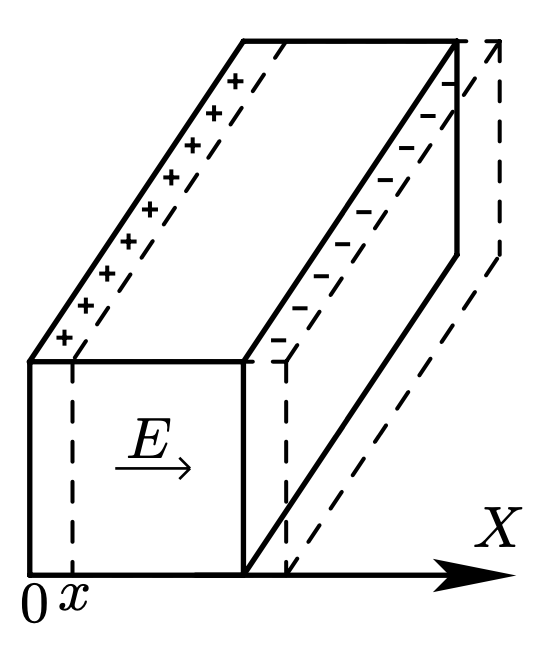
\includegraphics[width=0.6\linewidth]{1.png}
    \caption{\small{Параллелепипед с плотностью $n$}}
\end{wrapfigure}  

Теперь выделим параллелепипед с плотностью $n$ электронов (рис. 1), сместим их на $x$. 
Возникнут поверхностные заряды $\sigma = nex$, поле от которых будет придавать электронам ускорение:
\[\dfrac{d^2x}{dt^2}=-\dfrac{eE}{m}=-\dfrac{4\pi n e^2}{m}x.\]

Отсюда получаем плазменную (ленгмюровскую) частоту колебаний электронов:
\begin{equation}
    \omega_p = \sqrt{\dfrac{4\pi ne^2}{m}}.
\end{equation}

\subparagraph*{Одиночный зонд.}
При внесении в плазму уединённого проводника -- зонда -- с потенциалом, изначально равным потенциалу точки плазмы, в которую его помещают, на него поступают токи электроннов и ионов:
\begin{equation}
        I_{e0} = \dfrac{n \langle v_e \rangle}{4}eS,\quad I_{i0} = \dfrac{n \langle v_i \rangle}{4}eS,
\end{equation}
где $\langle v_e \rangle$ и $\langle v_i \rangle$ -- средние скорости электронов и ионов, $S$ -- площадь зонда, $n$ -- плотность электронов и ионов. 
Скорости электронов много больше скорости ионов, поэтому $I_{i0} \ll I_{e0}$. 
Зонд будет заряжаться до некоторого равновестного напряжения $-U_f$ -- плавающего потенциала.\\

\begin{wrapfigure}{r}{0.4\linewidth}
    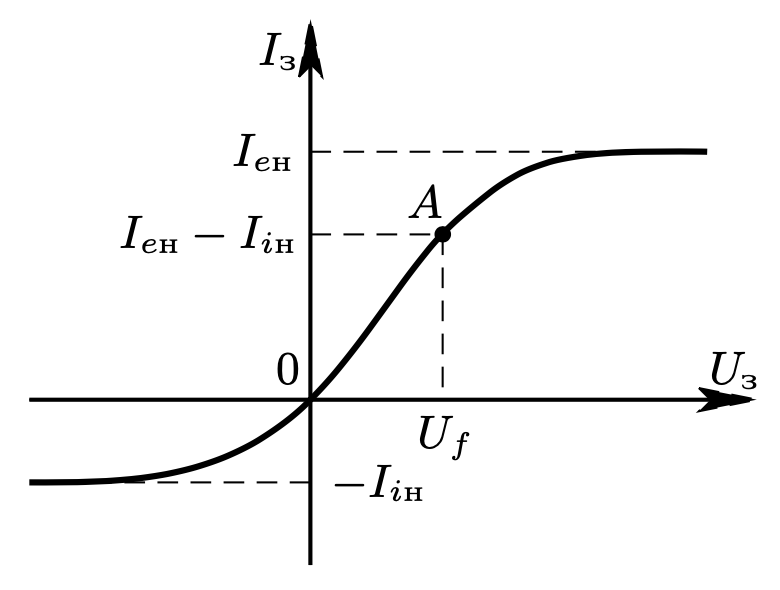
\includegraphics[width=\linewidth]{2.png}
    \caption{\small{Вольт-амперная характеристика одиночного зонда}}
\end{wrapfigure}  

В равновесии ионный ток мало меняется, а электронный имеет вид
\[I_e = I_0 \exp\left( -\dfrac{eU_f}{kT_e} \right).\]

Будем подавать потенциал $U_\text{з}$ на зонд и снимать значение зондового тока $I_\text{з}$. 
Максимальное значение тока $I_{e\text{н}}$ -- электронный ток насыщения, а минимальное $I_{i\text{н}}$ -- ионный ток насыщения. 
Значение из эмпирической формулы Бомона:
\begin{equation}
    I_{i\text{н}} = 0.4 neS \sqrt{\dfrac{2kT_e}{m_i}}.
\end{equation}

\subparagraph*{Двойной зонд.}
Двойной зонд -- система из двух одинаковых зондов, расположенных на небольшом расстоянии друг от друга, между которыми создаётся разность потенциалов, меньшая $U_f$. 
Рассчитаем ток между ними вблизи $I=0$. 
При небольших разностях потенциалов ионные токи на оба зонда близки к току насыщения и компенсируют друг друга, а значит величина результирующего тока полностью связана с разностью электронных токов. 
Пусть потенциалы на зондах
\[U_1 = -U_f + \Delta U_1,\]

\[U_2 = -U_f + \Delta U_2.\]

Между зондами $U = U_2 - U_1 = \Delta U_2 - \Delta U_1$.
Через первый электрод
\begin{equation}
    I_1 = I_{iн} + I_{e1} = I_{iн} - \dfrac{1}{4}neS\langle v_e\rangle \exp\left(-\dfrac{eU_f}{kT_e}\right)\exp\left(\dfrac{e\Delta U_1}{kT_e}\right)=I_{iн}\left(1 - \exp\left( \dfrac{e\Delta U_1}{kT_e} \right)\right).
\end{equation}

Аналогично через второй получим
\begin{equation}
    I_2 = I_{iн}\left(1 - \exp\left( \dfrac{e\Delta U_2}{kT_e} \right)\right)
\end{equation}
  
Из $(7)$ и $(8)$ с учётом последовательного соединение зондов ($I_1 = -I_2 = I)$:
\[\Delta U_1= \dfrac{kT_e}{e}\text{ln}\left(1 - \dfrac{I}{I_{iн}}\right)\]
\[\Delta U_2= \dfrac{kT_e}{e}\text{ln}\left(1 + \dfrac{I}{I_{iн}}\right)\]

\begin{wrapfigure}{l}{0.4\linewidth}
    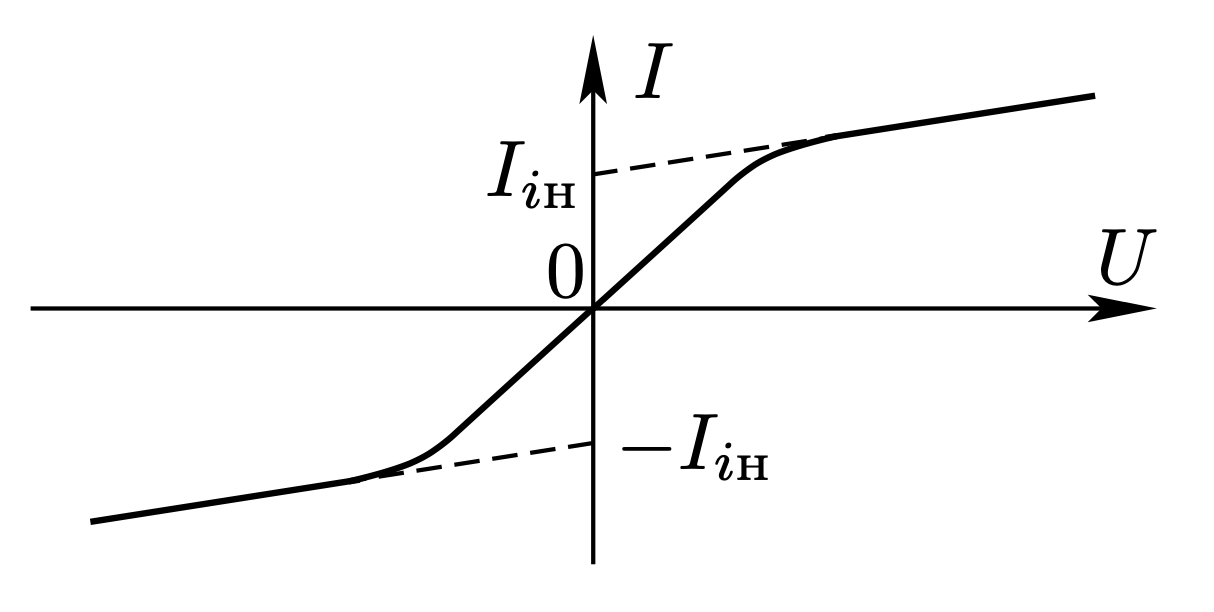
\includegraphics[width=\linewidth]{3.png}
    \caption{\small{Вольт-амперная характеристика двойного зонда}}
\end{wrapfigure}

Тогда итоговые формулы для разности потенциалов и тока

\begin{equation}
    U = \frac{kT_e}{e}\text{ln}\frac{1 - I/I_{iн}}{1 + I/I_{iн}}, \quad
    I = I_{iн} \tanh\dfrac{eU}{2kT_e}.
\end{equation}

Реальная зависимость выглядит несколько иначе и описывается формулой 

\begin{equation}
    I = I_{iн} \tanh\frac{eU}{2kT_e} + AU.
\end{equation}
Из этой формулы можно найти формулу для $T_e$: для $U=0$ мы найдём $I_{iн}$, продифференцируем в точке $U=0$ и с учётом $\tanh \alpha \approx \alpha$ при малых $\alpha$ и $A\rightarrow 0$ получим:
\begin{equation}
    kT_e = \dfrac{1}{2}\dfrac{eI_{iн}}{\dfrac{dI}{dU}|_{U=0}}.
\end{equation}

\subsection*{Экспериментальная установка}
Схема установки для исследования плазмы газового разряда в неоне представлена на рис. 1. 
Стеклянная газоразрядная трубка имеет холодный (ненагреваемый) полый катод, три анода и геттерный узел - стеклянный баллон, на внутреннюю поверхность которого напылена газопоглощающая плёнка (геттер). 
Трубка наполнена изотопом неона ${}^{22}$Ne при давлении 2 мм рт. ст. 
Катод и один из анодов (I или II) с помощью переключателя $П_1$ подключаются через балластный резистор $R_{\sigma}(\sim 450$ кОм $)$ к регулируемому высоковольтному источнику питания (ВИП) с выходным напряжением до 5 кВ.
\begin{figure}[H]
    \centering
    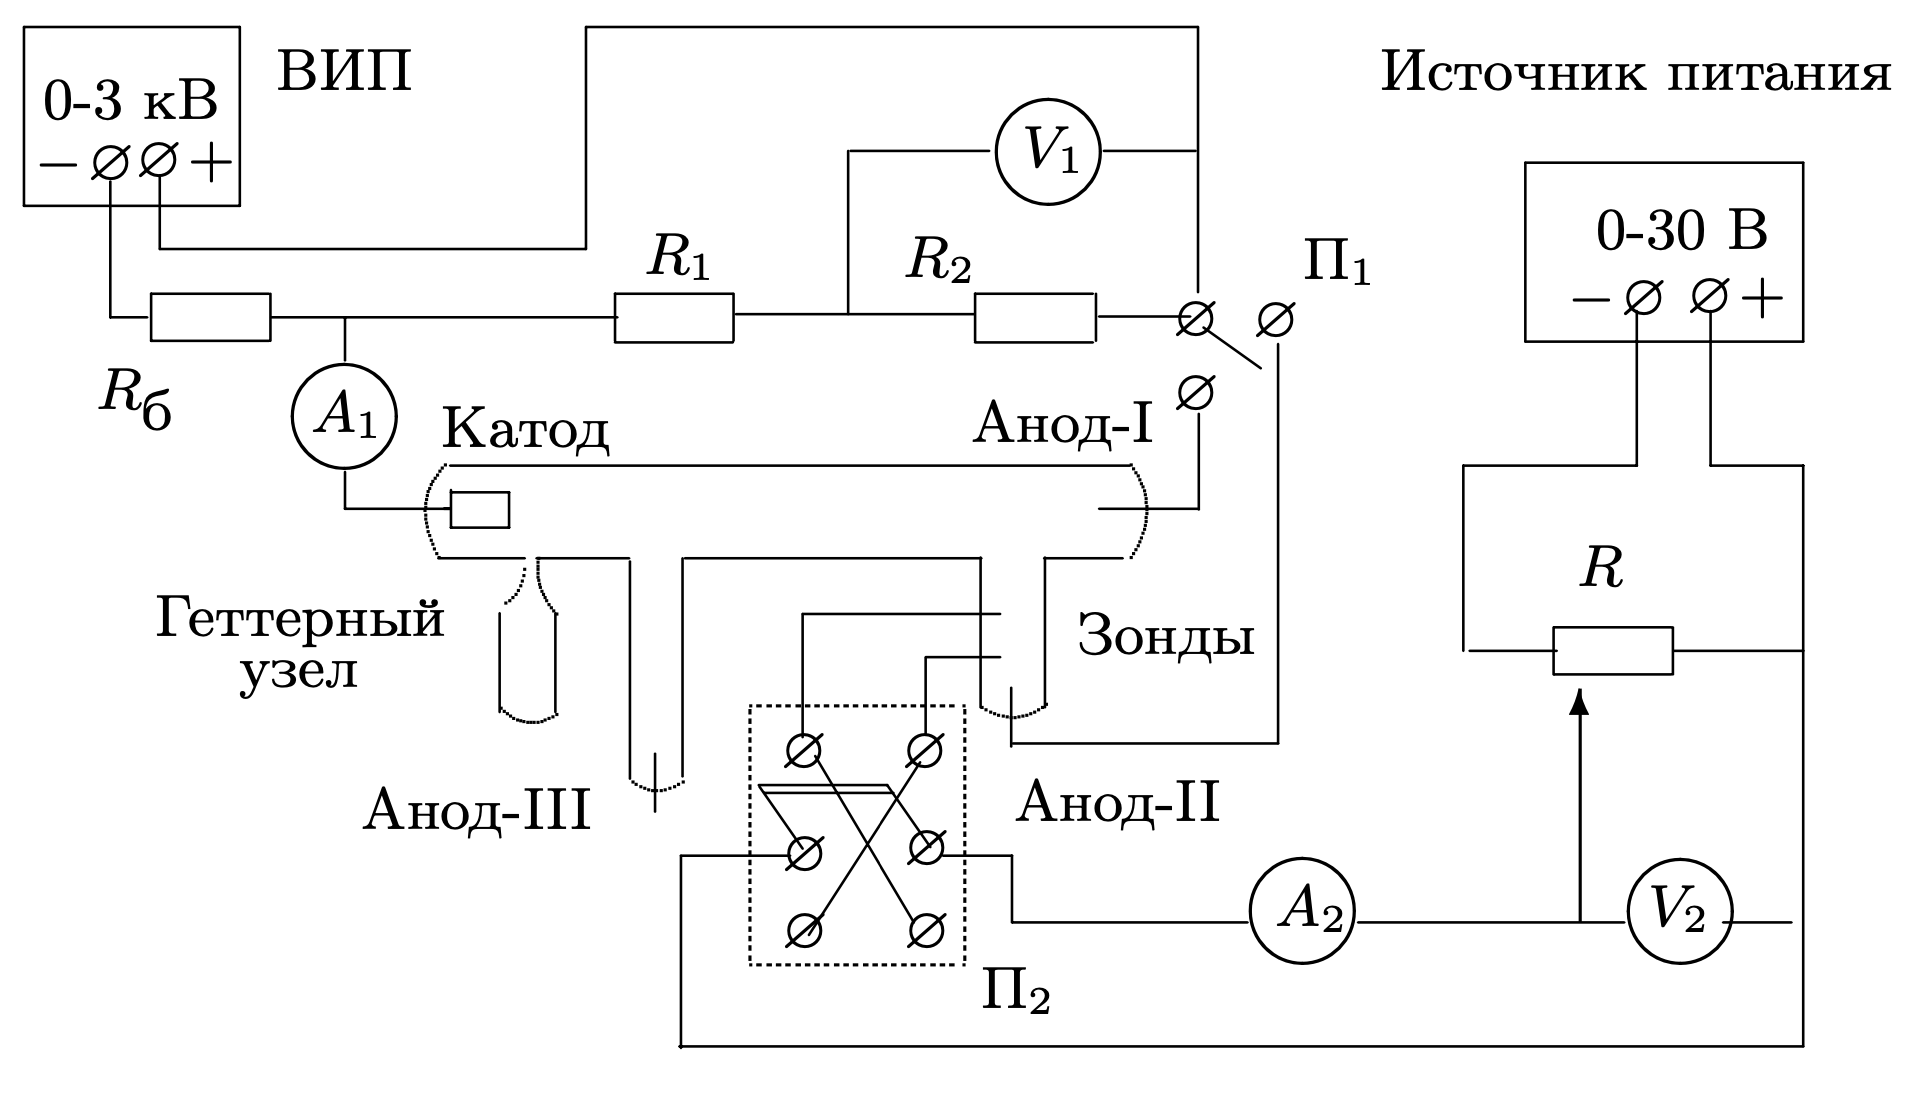
\includegraphics[width=0.7\linewidth]{scheme.png}
    \caption{Схема установки для исследования газового разряда}
\end{figure}

При подключении к ВИП анода-I между ним и катодом возникает газовый разряд. 
Ток разряда измеряется миллиамперметром $A_{1}$, а падение напряжения на разрядной трубке - цифровым вольтметром $V_{1}$ (мультиметром GDM), подключённым к трубке через высокоомный (25 МОм) делитель напряжения с коэффициентом $\left(R_{1}+R_{2}\right) / R_{2}=10$.

При подключении к ВИП анода-II разряд возникает в пространстве между катодом и анодом-II, где находится двойной зонд, используемый для диагностики плазмы положительного столба.

Зонды изготовлены из молибденовой проволоки диаметром $d=0.2$ мм и имеют длину $l=5.2$ мм. 
Они подключены к источнику питания GPS через потенциометр $R$. 
Переключатель $\Pi_{2}$ позволяет изменять полярность напряжения на зондах. 
Величина напряжения на зондах изменяется с помощью дискретного переключателя «$V$» выходного напряжения источника питания и потенциометра $R$, а измеряется цифровым вольтметром $V_{2}(\mathrm{GDM})$. 
Для измерения зондового тока используется мультиметр $A_{2}(\mathrm{GDM})$. 
Анод-III в нашей работе не используется. 

\subsection*{Результаты измерений и обработка данных}
Для начала, плавно увеличивая напряжение на ВИП определим напряжение зажигания разряда $U_{заж} = 31.68В$.

Теперь снимем зависимость напряжения разряда $U_p$ от его тока $I_p$ как при его увеличении, так и при убывании (табл. 1).

\begin{table}[H]
\centering
    \begin{tabular}[]{|c|c|c|c|c|c|c|c|c|c|c|c|c|c|c|}
\hline
$I_p$, дел         & 1.5   & 2.0   & 2.5   & 3     & 3.5   & 4     & 4.5   \\ \hline
$U_p\downarrow$, В & 31.69 & 30.44 & 28.38 & 27.65 & 27.25 & 27.15 & 27.18 \\ \hline
$U_p\uparrow$, В   & 31.58 & 29.37 & 28.11 & 27.56 & 27.23 & 27.16 & 27.18 \\ \hline
\end{tabular}
    \caption{Вольт-амперная характеристика разряда}
\end{table}

Изобразим полученные данные на графике (рис. 5)
\begin{figure}[H!]
    \centering
    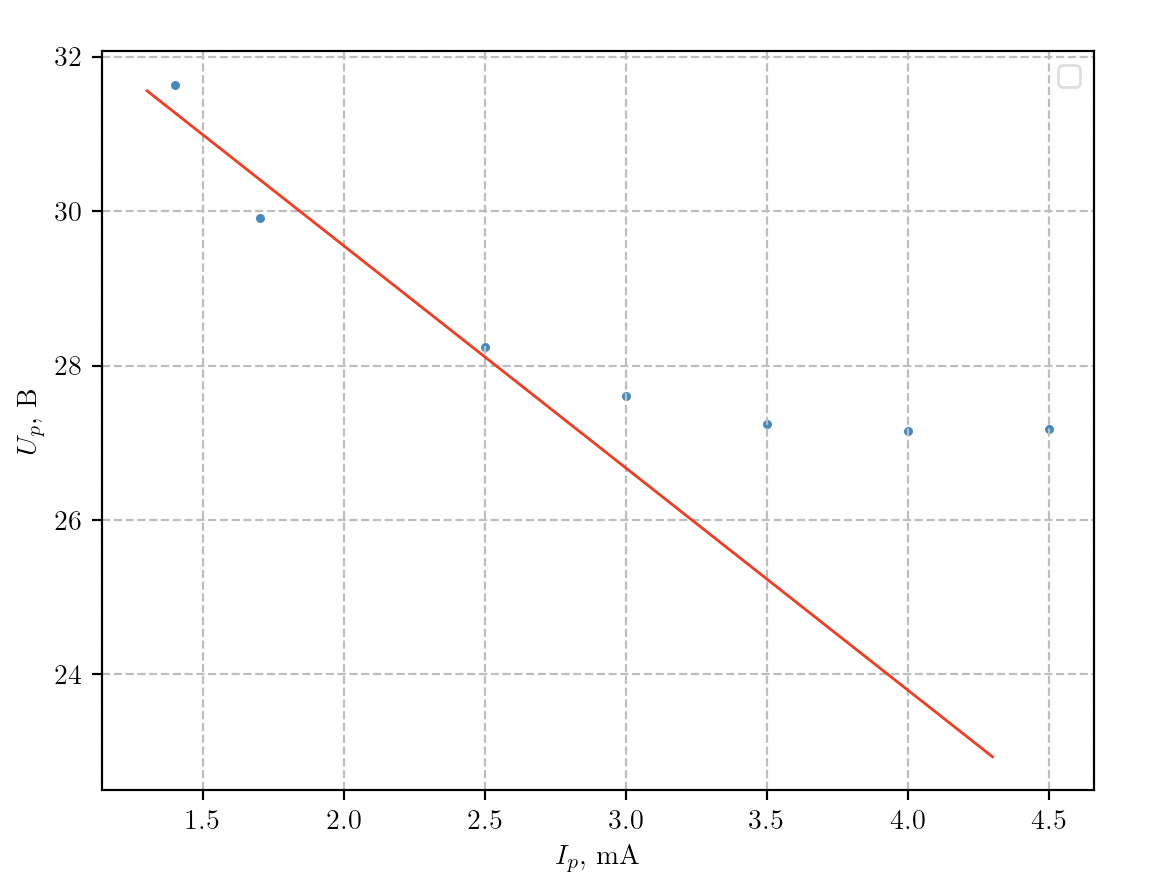
\includegraphics[width=0.6\linewidth]{1graph.png}
    \caption{ВАХ рязряда}
\end{figure}
Максималльное дифференциальное сопротивлние заряда $R_{диф} = (5.9 \pm 0.2) \cdot 10^3$ Ом 
 
4) $GPS :U_2=25, GDM: U=24.98$

Проведем серию измерений для вольт-амперной характеристики двойного зонда при различных разрядных токах (табл. 2).  
\begin{table}[H]
    \centering
    \resizebox{\textwidth}{!}{
    \begin{tabular}[]{|c|c|c|c|c|c|c|c|c|c|c|c|}
        \hline
        \multicolumn{12}{|c|}{$I_p = 5$ мА} \\        \hline

        $U_з$, В                          & 25.081                      & 22.006                      & 18.079                     & 16.009 & 13.019 & 10.014 & 8.060 & 6.030 & 4.007 & 1.997 & 0.052 \\ \hline
$I_з$, мкА                        & 120.20                      & 117.17                      & 114.15                     & 110.51 & 105.10 & 96.53  & 88.30 & 77.24 & 60.83 & 46.01 & 27.36 \\ \hline
$-U_з$, В                         & 25.064                      & 22.002                      & 19.010                     & 16.040 & 13.043 & 10.071 & 8.053 & 6.022 & 4.006 & 1.986 & 0.014 \\ \hline
\multicolumn{1}{|l|}{$-I_з$, мкА} & \multicolumn{1}{l|}{104.11} & \multicolumn{1}{l|}{100.86} & \multicolumn{1}{l|}{97.73} & 94.01  & 88.11  & 78.39  & 68.45 & 55.01 & 38.19 & 19.26 & 0.73  \\ \hline

        \multicolumn{12}{|c|}{$I_p = 4$ мА} \\        \hline

$U_з$, В                          & 25.068                     & 22.105                     & 19.010                     & 16.094 & 13.028 & 10.224 & 8.028 & 6.112 & 4.060 & 1.996 & 0.028 \\ \hline
$I_з$, мкА                        & 92.48                      & 89.86                      & 87.25                      & 84.08  & 80.25  & 75.37  & 68.72 & 60.50 & 48.76 & 33.92 & 17.46 \\ \hline
$-U_з$, В                         & 25.069                     & 22.064                     & 19.102                     & 16.119 & 13.025 & 10.193 & 8.018 & 6.162 & 4.121 & 2.019 & 0.030 \\ \hline
\multicolumn{1}{|l|}{$-I_з$, мкА} & \multicolumn{1}{l|}{75.98} & \multicolumn{1}{l|}{73.44} & \multicolumn{1}{l|}{71.02} & 68.31  & 64.33  & 57.87  & 49.80 & 40.17 & 26.55 & 9.84  & -7.43 \\ \hline

        \multicolumn{12}{|c|}{$I_p = 3$ мА} \\
        \hline
        $U_з$, В                          & 25.065                     & 21.977                     & 19.012                     & 16.002 & 19.150 & 10.024 & 8.092 & 6.065 & 4.097 & 1.997 & 0.019 \\ \hline
$I_з$, мкА                        & 69.52                      & 67.35                      & 65.31                      & 63.17  & 60.74  & 56.61  & 52.44 & 46.02 & 37.43 & 25.67 & 12.47 \\ \hline
$-U_з$, В                         & 25.068                     & 22.035                     & 19.009                     & 16.129 & 13.040 & 10.050 & 8.086 & 6.026 & 4.006 & 2.154 & 0.018 \\ \hline
\multicolumn{1}{|l|}{$-I_з$, мкА} & \multicolumn{1}{l|}{53.36} & \multicolumn{1}{l|}{51.52} & \multicolumn{1}{l|}{49.74} & 48.00  & 45.55  & 40.83  & 35.54 & 27.52 & 17.21 & 5.81  & -8.84 \\ \hline
        \multicolumn{12}{|c|}{$I_p = 2$ мА} \\
        \hline
        $U_з$, В                          & 25.069                     & 22.129                     & 19.174                     & 16.212 & 13.041 & 10.030 & 8.006 & 6.084 & 4.084 & 2.051 & 0.018 \\ \hline
$I_з$, мкА                        & 46.43                      & 44.91                      & 43.39                      & 41.83  & 40.09  & 37.57  & 34.81 & 30.94 & 25.28 & 17.72 & 8.54  \\ \hline
$-U_з$, В                         & 25.069                     & 22.046                     & 18.983                     & 16.006 & 13.058 & 10.028 & 8.065 & 5.990 & 4.143 & 2.037 & 0.020 \\ \hline
\multicolumn{1}{|l|}{$-I_з$, мкА} & \multicolumn{1}{l|}{33.01} & \multicolumn{1}{l|}{31.87} & \multicolumn{1}{l|}{30.76} & 29.68  & 28.33  & 25.48  & 22.19 & 17.03 & 10.82 & 2.03  & -7.33 \\ \hline

\multicolumn{12}{|c|}{$I_p = 1$ мА} \\
        \hline
       $U_з$, В                          & 25.069                     & 22.135                     & 19.076                     & 16.085 & 12.995 & 10.018 & 8.051 & 6.020 & 4.186 & 2.040 & 0.017 \\ \hline
$I_з$, мкА                        & 24.85                      & 23.94                      & 23.00                      & 22.08  & 21.04  & 19.57  & 18.04 & 15.81 & 13.12 & 9.10  & 4.59  \\ \hline
$-U_з$, В                         & 25.069                     & 22.076                     & 19.010                     & 16.041 & 13.005 & 10.032 & 8.072 & 6.039 & 4.091 & 2.065 & 0.012 \\ \hline
\multicolumn{1}{|l|}{$-I_з$, мкА} & \multicolumn{1}{l|}{15.91} & \multicolumn{1}{l|}{15.47} & \multicolumn{1}{l|}{15.01} & 14.54  & 13.90  & 12.40  & 10.59 & 7.90  & 4.55  & 0.36  & -4.33 \\ \hline
    \end{tabular}}
    \caption{Зондовые характеристики при разных токах}
\end{table}

Теперь отобразим данные на графиках и определим $I_{iн}$ и производную в нуле.

\begin{figure}[H]
    % \centering
    \subfigure[ВАХ двойного зонда при $I_p = 5$ мА]{
        \begin{minipage}{0.5\linewidth}
            \centering
            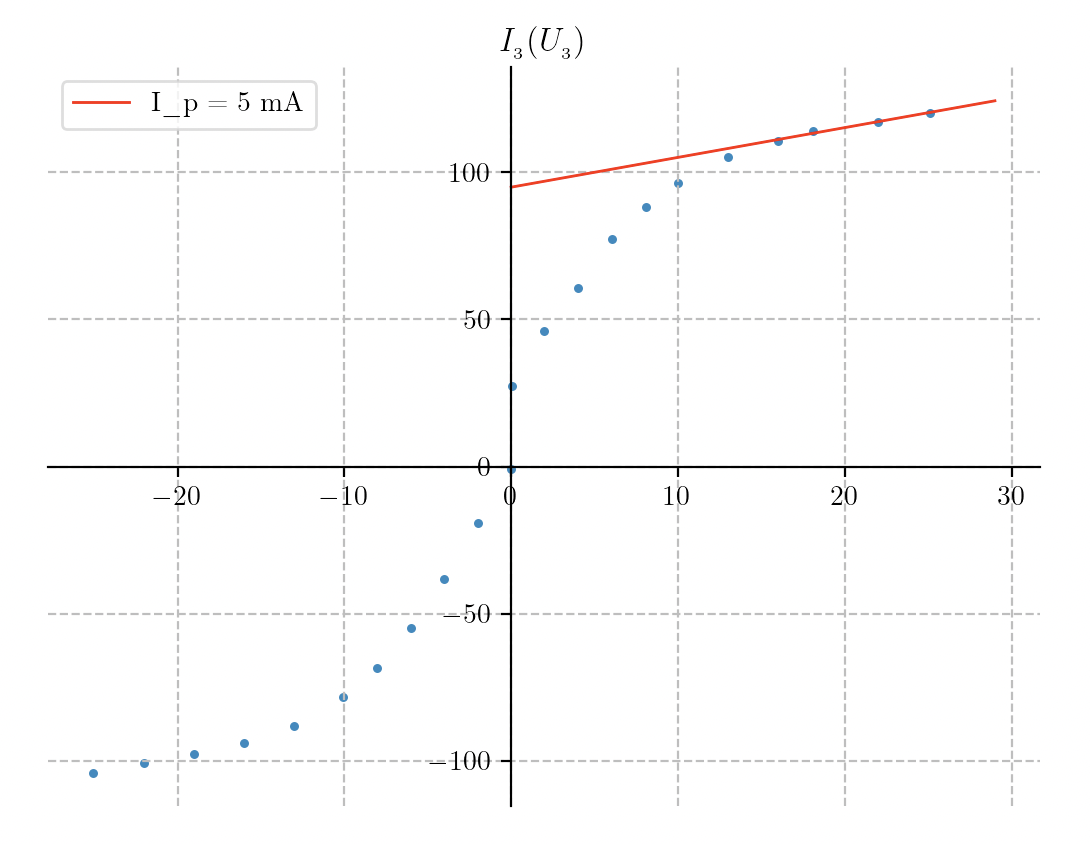
\includegraphics[width=\linewidth]{5ma.png}
        \end{minipage}
    }
    \subfigure[ВАХ двойного зонда при $I_p = 4$ мА]{
        \begin{minipage}{0.5\linewidth}
            \centering
            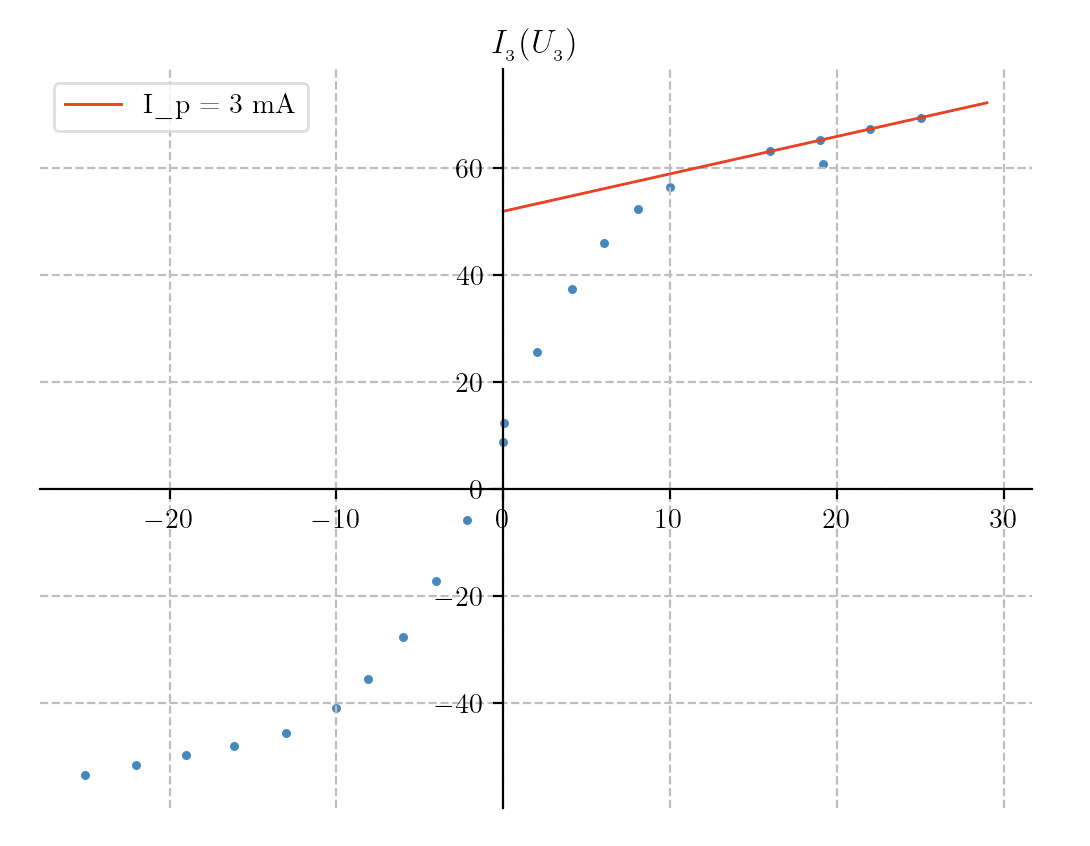
\includegraphics[width=\linewidth]{4ma.png}
        \end{minipage}
    }
\end{figure}

\begin{figure}[H]
    % \centering
    \subfigure[ВАХ двойного зонда при $I_p = 3$ мА]{
        \begin{minipage}{0.5\linewidth}
            \centering
            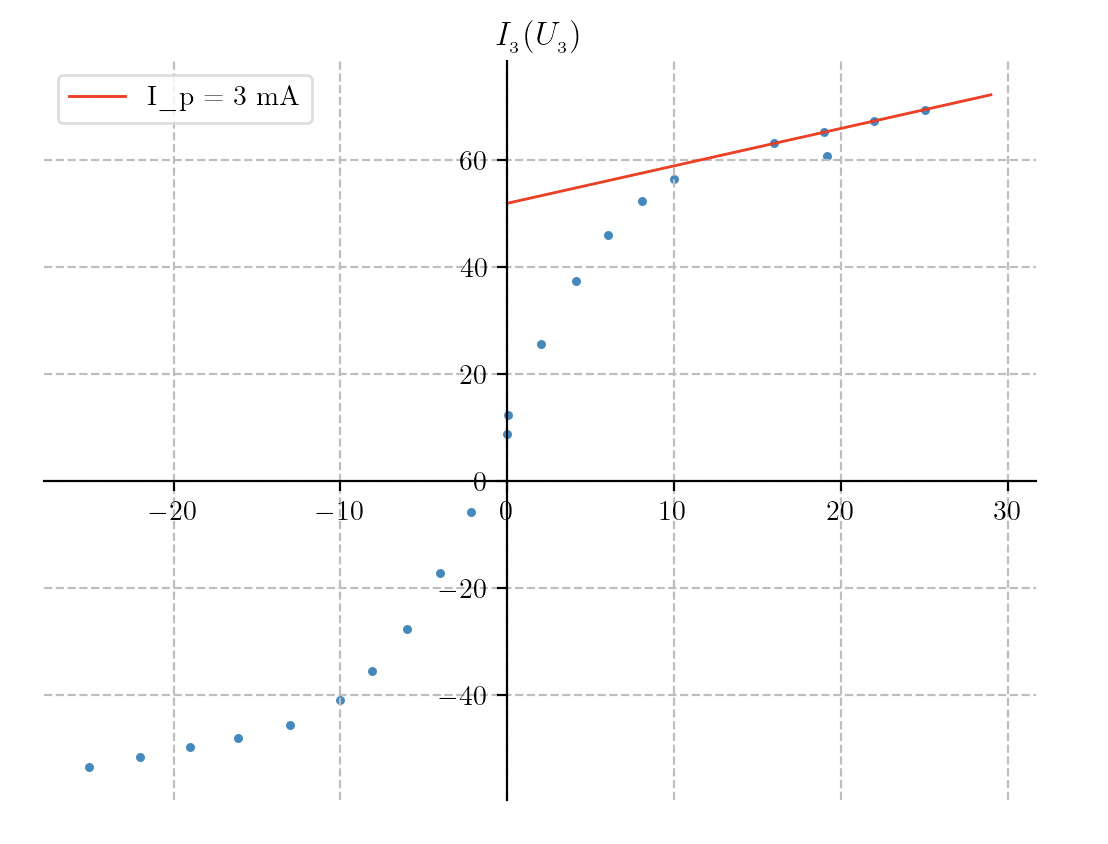
\includegraphics[width=\linewidth]{3ma.png}
        \end{minipage}
    }
    \subfigure[ВАХ двойного зонда при $I_p = 2$ мА]{
        \begin{minipage}{0.5\linewidth}
            \centering
            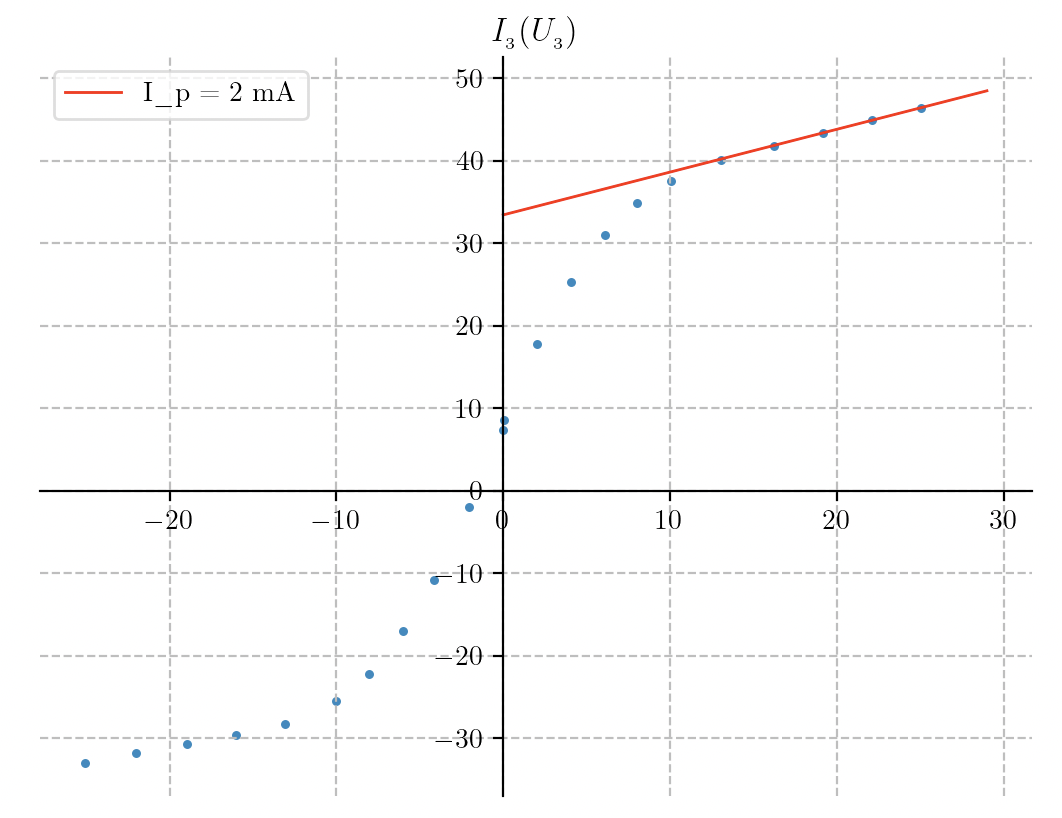
\includegraphics[width=\linewidth]{2ma.png}
        \end{minipage}
    }
\end{figure}

\begin{figure}[H]
    \centering
    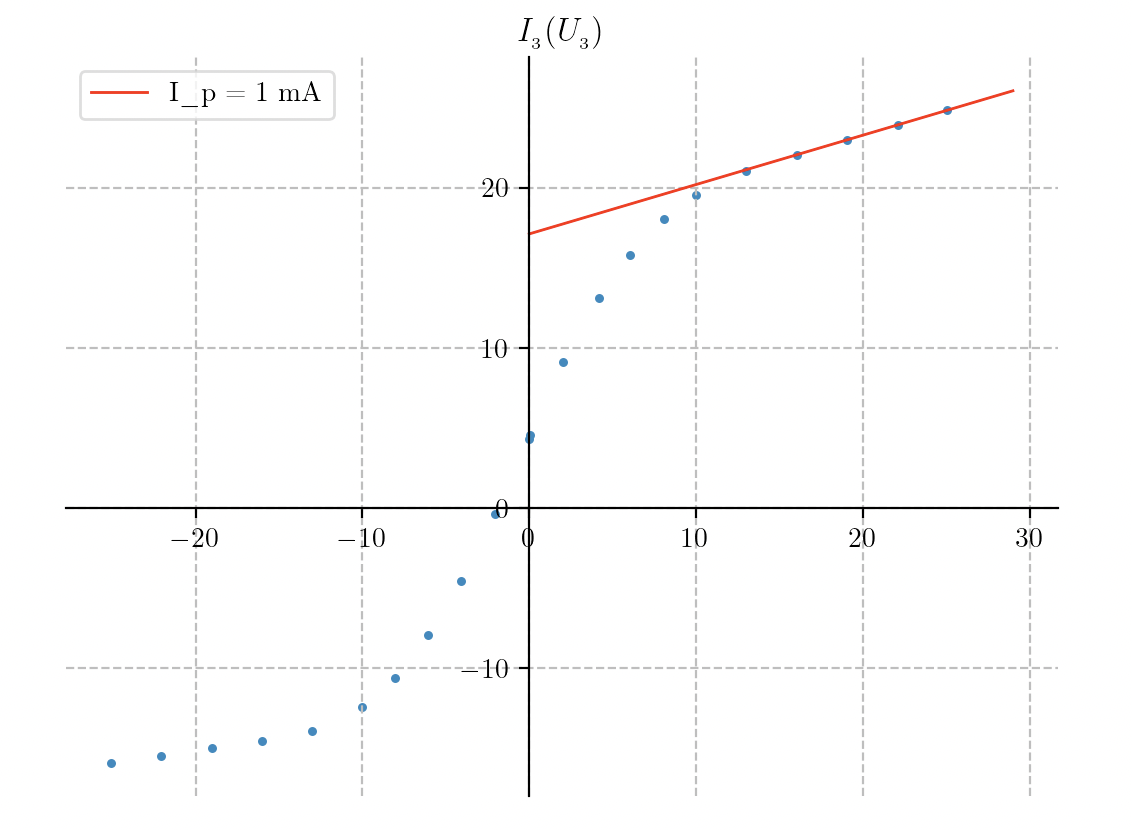
\includegraphics[width=0.4\linewidth]{1ma.png}
    \caption{ВАХ двойного зонда при $I_p = 1$ мА}
\end{figure}

Также изобразим все ВАХ на одном графике (рис. 7)

\begin{figure}[H]
    \centering
    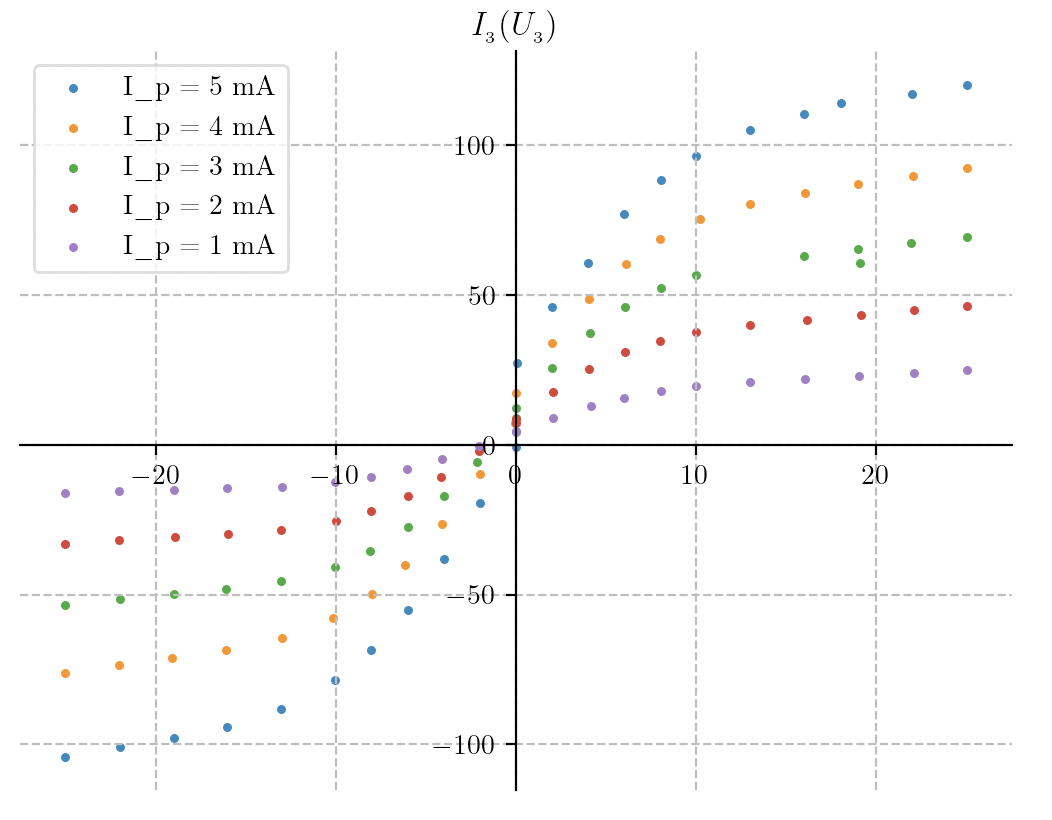
\includegraphics[width=0.7\linewidth]{all_ma.png}
    \caption{ВАХ двойного зонда при различных токах}
\end{figure}

% $\dfrac{dI}{dU}|_{U=0}(5мА) = (2.87\pm 0.03) \cdot 10^{-8} А/В$,\quad $\dfrac{dI}{dU}|_{U=0}(3мА) = (1.1\pm 0.2) \cdot 10^{-7} А/В$,

% $\dfrac{dI}{dU}|_{U=0}(1.5мА) = (2.7\pm 0.3) \cdot 10^{-7} А/В$, 
 
% Теперь можем из (12) вычислить температуру электронов $T_e = (1.8 \pm 0.1) \cdot 10^7$ К, $(2.4 \pm 0.5) \cdot 10^6$ К и $(4.4 \pm 0.6) \cdot 10^5$ К соответсвенно.

Теперь из (12) можем вычислить температуру электронов $T_e$.
% $T_e = (1.7 \pm 0.1) \cdot 10^4$ К, $T_e = (2.4 \pm 0.5) \cdot 10^4$ К, $T_e = (3.9 \pm 0.1) \cdot 10^4$ К соответсвенно.
% \vspace{0.3cm}

Также из (7) расчитаем концентрацию ионов $n_i$, полагая ее равной концентрации электронов $n_e$.
% $n_e = (6.0 \pm 0.5) \cdot 10^{13} м^{-3}$, $n_e = (2.6 \pm 0.3) \cdot 10^{13} м^{-3}$, $n_e = (9.1 \pm 0.3) \cdot 10^{12} м^{-3}$.
% \vspace{0.3cm}

Из (5) получим плазменную частоту колебаний электронов $\omega_p$
% = (4.6 \pm 0.2)\cdot 10^3 {рад \over с}$, $\omega_p = (3.0 \pm 0.2)\cdot 10^3 {рад \over с}$, $\omega_p = (1.8 \pm 0.1)\cdot 10^3 {рад \over с}$.
% \vspace{0.3cm}

\begin{figure}[H]
    \centering
    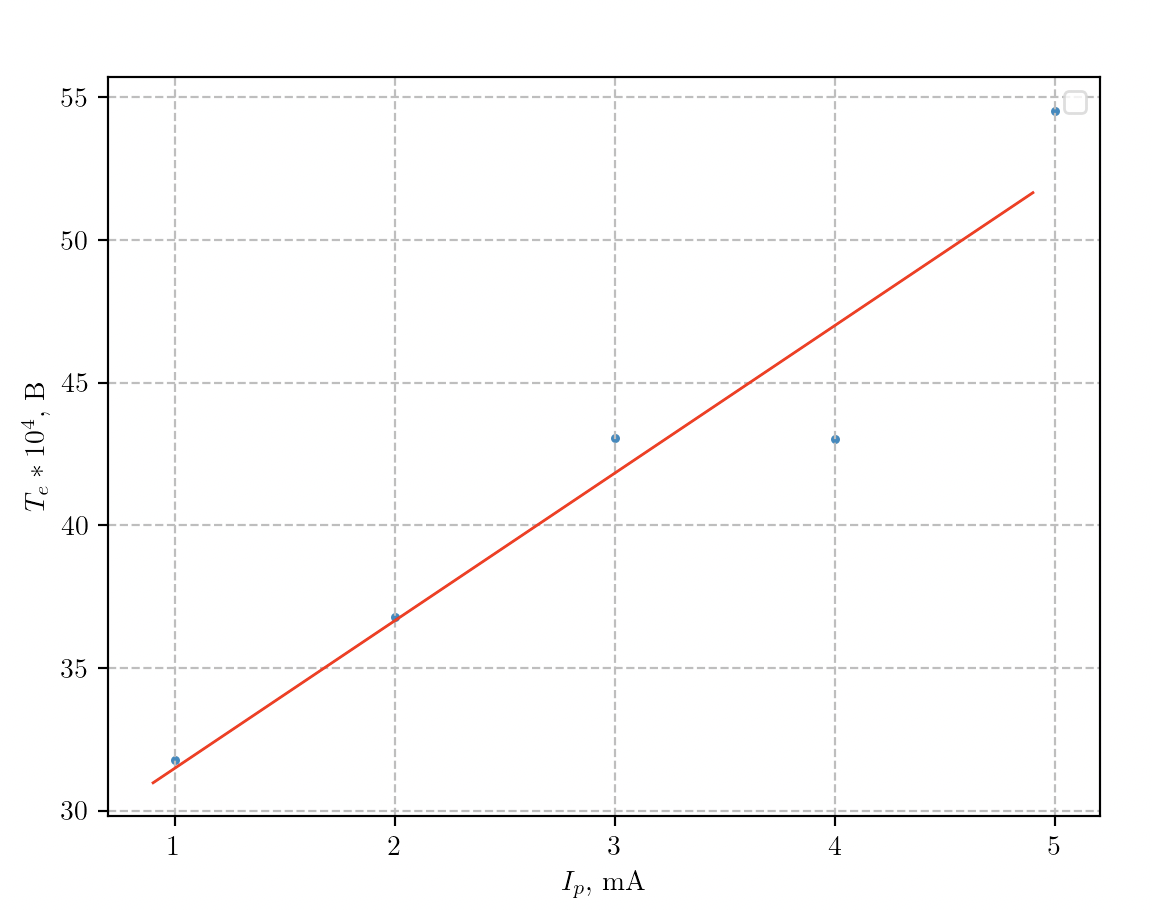
\includegraphics[width=0.5\linewidth]{Te(Ip).png}
    \caption{График завиисимости $T_e(I_p)$}
\end{figure}

\begin{figure}[H]
    \centering
    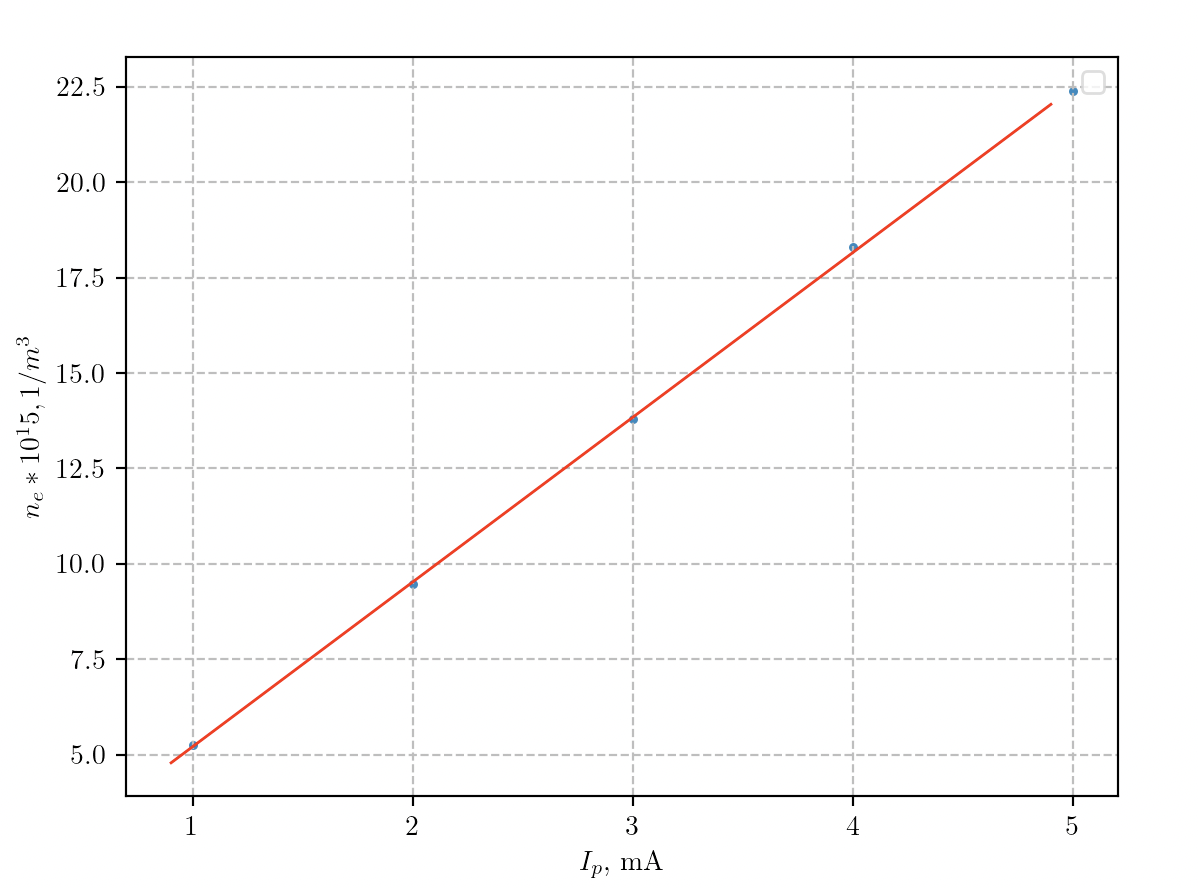
\includegraphics[width=0.5\linewidth]{ne(Ip).png}
    \caption{График завиисимости $n_e(I_p)$}
\end{figure}

Расчитаем электронную поляризационную длину $r_{D_e}$, радиус Дебая $r_{D}$ и по формуле (4)  вычислим среднее число ионов в сфере такого радиуса $<N_D>$.
% $r_{D_e} = (1.5 \pm) \cdot 10^{-4}$ м, $r_{D_e} = (1.5 \pm) \cdot 10^{-4}$ м
Степень ионизации $\alpha$ получим по соотношению $\alpha = n_i/n$, где $n$ -- общее число частиц в единице объема (давление $P=nkT_i\approx 1$мбар). 
Все результаты занесем в таблицу 3.

\begin{table}[H]
    \centering
    \resizebox{\textwidth}{!}{
    \begin{tabular}{|l|l|l|l|l|l|l|l|l|}
        \hline
        $I_p$, мА& $I_н$, мА& $\dfrac{dI}{dU}|_{U=0}$, $\frac{мА}{В}$&$T_e, 10^4$, К&$n_e, 10^{15} м^{-3}$&$\omega_p, 10^3{рад \over сек}$&$r_Dе, 10^{-4}см$&$<N_D>,10^4  частиц$&$\alpha, 10^{-10}$ \\
        \hline
        5               & 95\pm 4          & 1,01\pm 0,5                      & 54 \pm 3                                  & 22,4                                                                 & 8,9         & 7,6 \pm 0,1                                       & 41 \pm 1                 & 8,37\pm 0,6                                      \\ \hline
        4               & 69 \pm 3        & 0,93\pm 0,4                       & 43 \pm 3                                  & 18,3                                                                 & 8,0         & 8,3 \pm 0,1                                       & 45 \pm 2                 & 6,81\pm 0,5                                       \\ \hline
        3               & 52\pm 3         & 0,70\pm 0,4                       & 43 \pm 3                                  & 13,8                                                                 & 6,9         & 9,6 \pm 0,1                                       & 52 \pm 2                  & 5,12\pm 0,05                                       \\ \hline
        2               & 33\pm 2         & 0,52 \pm 0,2                      & 36\pm 2                                   & 9,5                                                                  & 5,7         & 11,7 \pm 0,1                                      & 62 \pm 2                  & 3,52\pm 0,04                                       \\ \hline
        1               & 17\pm 2          & 0,31\pm 0,2                       & 32 \pm 2                                  & 5,24                                                                 & 4,3         & 15,6 \pm 0,1                                      & 84 \pm 3                 & 1,95 \pm 0,04                                      \\ \hline
    \end{tabular}}
    \caption{Вычисленные характеристики}
\end{table}

\subsection*{Подведение итогов}
В ходе работы снята вольт-амперная характеристика тлеющего разряда и зондовые характеристики при разных токах разряда.
По результатам измерений рассчитаны концентрация и температура электронов в плазме, плазменная частота, поляризационная длина, дебаевский радиус экранирования и степень ионизации.

По полученным значениям характеристик можно заключить, что плазма не является квазинейтральной, т.к. электронная поляризационная длина не сильно превосходит дебаевский радиус.
\end{document}